\documentclass{standalone}
\usepackage{pgfplots}
\pgfplotsset{compat=1.6}

\pgfplotsset{soldot/.style={color=black,only marks,mark=*}} \pgfplotsset{holdot/.style={color=black,fill=white,only marks,mark=*}}

\begin{document}

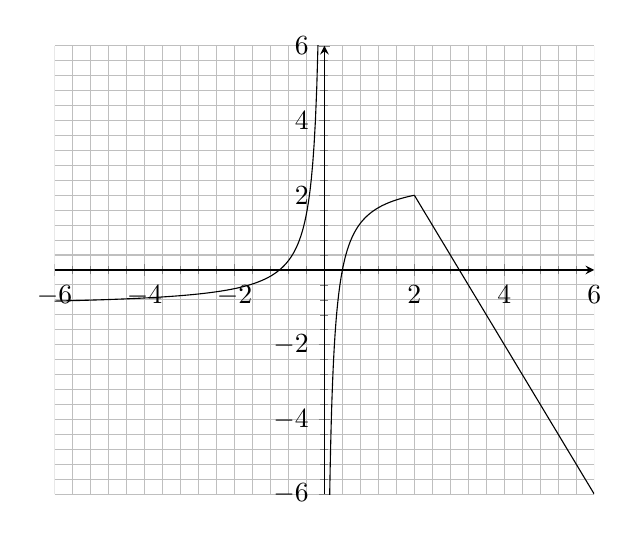
\begin{tikzpicture}
\begin{axis}[minor tick num=4,axis lines=middle,grid=both,xmin=-6,xmax=6,ymin=-6,ymax=6,samples=200]
\addplot[domain=-6:-0.05,black] {-1 - x^(-1)};
\addplot[domain=0.05:2,black] {2.5 - x^(-1)};
\addplot[domain=2:6,black] {6-2*x};
%\addplot[holdot] coordinates{(0,0)(4,4)(6,-5)};
%\addplot[soldot] coordinates{(4,8)(6,6)(10,-5)};
\end{axis}
\end{tikzpicture}

\end{document}
